\ifx \globalmark \undefined %% This is default.
	\documentclass[twoside,openright,11pt,a4paper]{report}

%\compiler avec xelatex
%\usepackage[applemac]{inputenc}
\usepackage[T1]{fontenc}
\usepackage[utf8]{inputenc} %latin1 est possible
%\usepackage[latin1]{inputenc} %latin1 est possible
\usepackage[UKenglish]{babel}
\usepackage{lettrine}

%\usepackage[text={13cm,20cm},centering]{geometry}
\usepackage [squaren, Gray, mediumqspace]{SIunits}
\usepackage [top=2cm, bottom=2cm, left=2cm, right=2cm ]{geometry}

\renewcommand{\familydefault}{cmss}
\addto\captionsenglish{ \renewcommand\chaptername{Solutions of Chapte}}

\usepackage{graphicx}
\usepackage{amsmath}
\usepackage{amsfonts}
\usepackage{amssymb}
\usepackage{amsthm}
\usepackage{bm}
\usepackage{color}

\newcommand{\real}{\mathbb{R}}
\newcommand{\mb}{\mathbf}
\newcommand{\bos}{\boldsymbol}

\def \RR {I \! \! R}

\newcommand{\e}{\begin{equation}}  
\newcommand{\ee}{\end{equation}}
\newcommand{\eqn}{\begin{eqnarray}} 
\newcommand{\eeqn}{\end{eqnarray}} 
\newcommand{\eqnn}{\begin{eqnarray*}} 
\newcommand{\eeqnn}{\end{eqnarray*}} 

\newcommand{\bpm}{\begin{pmatrix}}
\newcommand{\epm}{\end{pmatrix}}

%\newcommand{\{\c c}}{\c c}

\newcommand{\bma}{\left(\begin{array}}
\newcommand{\ema}{\end{array}\right)} 
\newcommand{\hh}{\hspace{2mm}}
\newcommand{\hd}{\hspace{5mm}}
\newcommand{\hu}{\hspace{1cm}}
\newcommand{\vv}{\vspace{2mm}}
\newcommand{\vd}{\vspace{5mm}}
\newcommand{\vm}{\vspace{-2mm}}
\newcommand{\teq}{\triangleq}
%\newcommand{\qedb}{\,$\Box$}
\newcommand{\blanc}{$\left. \right.$}
\newcommand{\frts}[2]%
         {\frac{{\textstyle #1}}{{\textstyle #2}}}

\newcommand{\bindex}[3]%
{
\renewcommand{\arraystretch}{0.5}
\begin{array}[t]{c}
#1\\
{\scriptstyle #2}\\
{\scriptstyle #3}
\end{array}
\renewcommand{\arraystretch}{1}
}

\theoremstyle{definition}
\newtheorem{exemple}{{\bf Exemple}}[chapter]
\newtheorem{theoreme}[exemple]{{\bf Th{é}or{è}me}}
\newtheorem{propriete}[exemple]{{\bf Propri{é}t{é}}}
\newtheorem{definition}[exemple]{{\bf D{é}finition}}
\newtheorem{remarque}[exemple]{{\bf Remarque}}
\newtheorem{remarques}[exemple]{{\bf Remarques}}
\newtheorem{lemme}[exemple]{{\bf Lemme}}
\newtheorem{hypothese}[exemple]{{\bf Hypoth{è}se}}
\newtheorem{exercice}{{\bf Exercice}}[chapter]

\newcommand{\xqedhere}[2]{%
 \rlap{\hbox to#1{\hfil\llap{\ensuremath{#2}}}}}

\newcommand{\xqed}[1]{%
 \leavevmode\unskip\penalty9999 \hbox{}\nobreak\hfill
 \quad\hbox{\ensuremath{#1}}}

\newcommand{\gf}{\fg\,\,}

\newcommand{\cata}[1] %
     {\renewcommand{\arraystretch}{0.5}
     \begin{array}[t]{c} \longrightarrow \\ {#1} \end{array}
     \renewcommand{\arraystretch}{1}}

\usepackage[isu]{caption}
%\usepackage[font=small,format=plain,labelfont=bf,up,textfont=it,up]{caption}
\setlength{\captionmargin}{60pt}

\newcommand{\cqfd}
{%
\mbox{}%
\nolinebreak%
\hfill%
\rule{2mm}{2mm}%
\medbreak%
\par%
}

\pagestyle{headings}

\renewcommand{\sectionmark}[1]{%
\markright{\thesection.\ #1}{}}

\renewcommand{\chaptermark}[1]{%
\markboth{\chaptername\ \thechapter.\ #1}{}}

\makeatletter 
\def\@seccntformat#1{\csname the#1\endcsname.\;} 
\makeatother

\title{ {\Huge {\textbf{Modélisation et analyse  \\ \vspace{4mm} des systèmes dynamiques }}} \\ \vspace{4cm} G. Bastin}

%\title{ {\Huge {\textbf{Modelisation et analyse  \\ \vspace{4mm} des systemes dynamiques }}} \\ \vspace{4cm} G. Bastin}


\date{\today}
	\begin{document} %% Crashes if put after (one of the many mysteries of LaTeX?).
\else 
	\documentclass{standalone}
	\begin{document}
\fi
	
\graphicspath{ {images/} }

\setcounter{chapter}{2}
\chapter{Systèmes électriques et électromécaniques}
\chaptermark{Systèmes électriques et électromécaniques}\label{systelec}



\lettrine[lines=1]{\bf C}{}e chapitre traite de la modélisation de systèmes dont la dynamique est essentiellement caractérisée par la présence de courants électriques, c'est à dire par le mouvement de charges électriques dans des matériaux conducteurs (par exemple des fils métalliques). Nous étudierons tout d'abord la mise en équation du modèle d'état des réseaux électriques. Nous étudierons ensuite les systèmes électromécaniques (en particulier les machines électriques) qui combinent en une description unifiée les équations d'état des réseaux électriques avec celles des systèmes mécaniques telles que nous les avons présentées au chapitre précédent.




\section{Les systèmes électriques}

Un système  électrique est défini comme une boîte noire munie de bornes, qui sont des points de contact électriques chacun soumis à un voltage $V_i$ et laissant entrer un courant $I_i$ (voir fig.~\ref{fig:systemelec}).
\begin{figure}[t]
\begin{center}
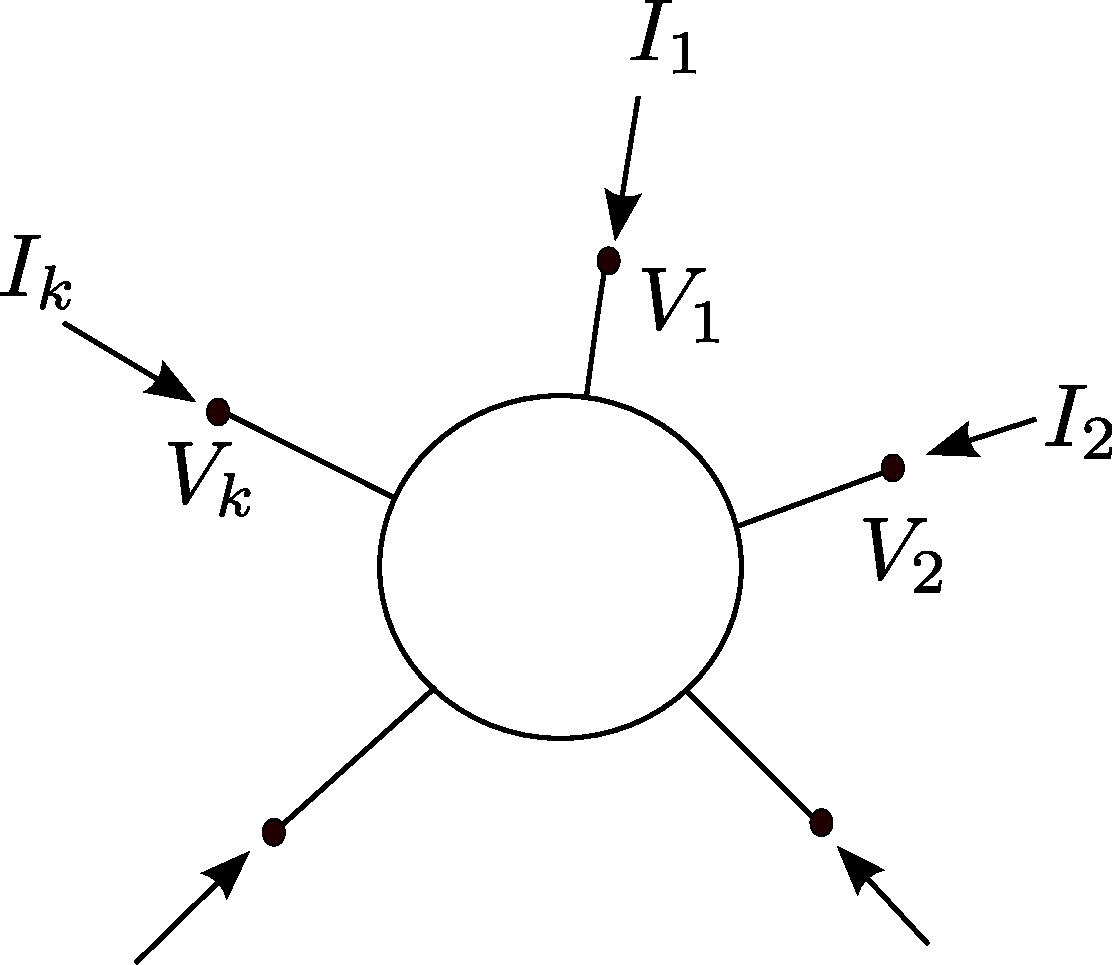
\includegraphics[width=7cm]{systemelec}
\caption{Système électrique}
\label{fig:systemelec}
\end{center}
\end{figure}

Le comportement du système est donné par l'ensemble de toutes les trajectoires $(I_1(t), V_1(t), I_2(t), V_2(t), \ldots, I_k(t), V_k(t))_{t \in \real}$ possibles pour le système. Cet ensemble de trajectoires possède des symétries. En effet, les lois de l'électricité nous enseignent que les potentiels ne sont définis qu'à une constante près. Autrement dit, si $(I_1(t), V_1(t), I_2(t), V_2(t), \ldots, I_k(t), V_k(t))_{t \in \real}$ est une trajectoire possible, alors $(I_1(t), V_1(t)+V, I_2(t), V_2(t)+V, \ldots, I_k(t), V_k(t)+V)_{t \in \real}$ est également une trajectoire possible. De plus, dans la quasi-totalité des circuits réalisés aujourd'hui, il n'y a pas d'accumulation de charge électrique: le système reste neutre électriquement, ce qui implique que $I_1(t) + I_2(t) + \ldots + I_k(t)=0$ à tout instant $t$.

Notons que la puissance transmise au circuit par l'environnement au temps $t$ est $\sum_i V_i(t) I_i(t)$. Cette formule a un sens physique univoque grâce aux deux relations ci-dessus: translater tous les voltages d'une constante ne modifie pas la puissance reçue. 


Les circuits électriques les plus simples ont seulement deux bornes, nommés  pour cela dipôles. Dans ce cas, il suffit de deux variables pour caractériser les trajectoires: la différence de potentiel, ou tension, $v(t)=V_1-V_2$ et le courant $i(t)=I_1(t)=-I_2(t)$ (voir fig.~\ref{fig:dipole}). Les sens du courant et la tension sont choisis de manière conventionnelle.
\begin{figure}[t]
\begin{center}
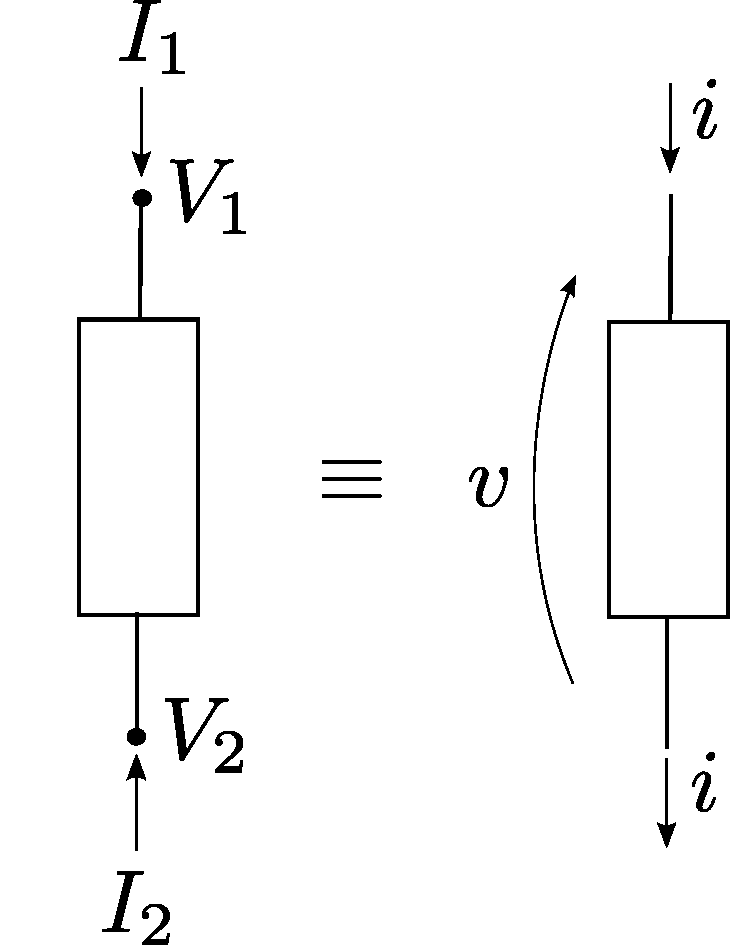
\includegraphics[width=5cm]{dipole2}
\caption{Dipôle électrique}
\label{fig:dipole}
\end{center}
\end{figure}
La tension représente donc l'énergie nécessaire pour déplacer une charge électrique unitaire à travers le dipôle.  On peut également avoir des tripôles (sytèmes à trois bornes, tels que les transistors) ou des quadrupôles (par exemple les transformateurs). 

Dans ce cours, 
nous ne considérons que les circuits dont le comportement 
(l'ensemble des trajectoires possibles) peut être décrit par un modèle d'état 
comme défini au Chapitre 1, où chaque variable extérieure (voltage ou courant) 
est pris, soit comme une entrée $u_i$, soit comme une sortie $y_i$. 
Les variables d'état peuvent être des voltages, courant, flux ou charges,
 comme on le verra. Ce type de modèle d'état cantonné aux équations différentielles est restrictif, en ce qu'il nous interdit par exemple de modéliser commodément les élément de délai, dont le comportement vérifie une équation de délai de type $y(t)=u(t-1)$ (donc non différentielle). 



\section{Dipôles élémentaires}


Nous considérons deux types de dip{ô}les élémentaires:
les impédances et les sources.
\begin{description}
\item{\bf Les impédances}
\begin{enumerate}
\item{\em Les résistances}. Les résistances sont des éléments qui transforment l'énergie électrique en chaleur. Elles sont représentées par
le symbole de la figure \ref{fig:impedances} et sont caractérisées
par une relation algébrique entre la tension $v(t)$ et le courant
$i(t)$ :
\eqnn
r(v(t), i(t)) = 0.
\eeqnn
\begin{figure}[t]
\begin{center}
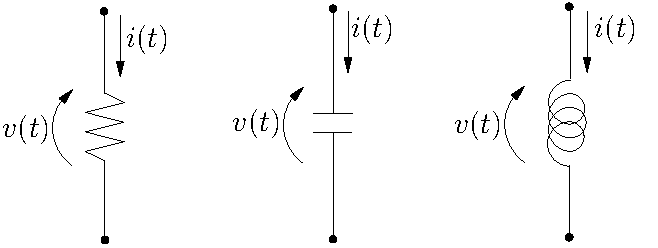
\includegraphics[width=9cm]{impedances}
\caption{Impédances : résistance, capacité, inductance}
\label{fig:impedances}
\end{center}
\end{figure}
Dans le cas d'une résistance linéaire, cette relation se
particularise comme suit (loi d'Ohm) :
\eqnn
v(t) = Ri(t).
\eeqnn
\item {\em Les capacités.} Les capacités sont des éléments qui accumulent les charges électriques. Elles sont représentées par le
symbole de la figure \ref{fig:impedances} et sont caractérisées par la
relation suivante entre la charge $Q(t)$ et le courant $i(t)$ :
\eqnn
i(t) = \frac{dQ(t)}{dt}.
\eeqnn
La charge $Q(t)$ est une fonction de la tension : $Q(v(t))$.  Cette relation peut aussi
s'écrire sous la forme suivante :
\eqnn
i(t) = c(v(t)) \frac{dv(t)}{dt} \;\;
\text{ où } \;\; c(v) \triangleq  \frac{\partial q}{\partial v}.
\eeqnn
Dans le cas d'une capacité linéaire, cette relation se
particu\-larise comme suit :
\eqnn
Q(t) = Cv(t) \;\; \text{ où } \;\; i(t) = C\frac{dv(t)}{dt}.
\eeqnn
\item{\em Les inductances.}  Les inductances sont des éléments qui emmagasinent l'énergie d'un champ magnétique. Elles sont représentées par le
symbole de la figure \ref{fig:impedances} et sont caractérisées, en vertu de
la loi de Faraday, par la relation suivante entre le flux magnétique $\phi(t)$ et la tension
$v(t)$ :
\eqn
v(t) = \frac{d \phi}{dt}. \label{definduc}
\eeqn
On dit que la tension $v(t)$ est {\it induite} par la variation de flux $\phi(t)$ d'où le nom d'inductance. D'une manière générale, cette variation de flux peut être produite par un matériau magnétique en mouvement dans les parages de l'inductance, ou encore par un courant électrique variable circulant dans un conducteur situé à proximité de l'inductance. Dans cette section, nous considérerons uniquement le cas particulier des {\it auto-inductances} où le flux est produit uniquement par le courant traversant le dipôle lui-même. Dans ce cas le flux est une fonction du courant :  $\phi(i(t))$ et la relation (\ref{definduc}) s'écrit aussi sous la forme suivante :
\eqnn
v(t) =  l(i(t)) \frac{di(t)}{dt}
\mbox{ où } l(i) \triangleq  \frac{\partial \phi}{\partial i}.
\eeqnn
Dans le cas d'une (auto)inductance linéaire, cette relation se
particularise comme suit :
\eqnn
\phi(t) = Li(t) \;\; \mbox{ où } v(t) = L \frac{di(t)}{dt}.
\eeqnn
\end{enumerate}
\item{\bf Les sources}
\begin{enumerate}
\item {\em Les sources de tension} représentées par le symbole de
la figure \ref{fig:sources} sont des dip{ô}les définis par la
tension $v(t)$ indépendam\-ment du courant qu'ils débitent.
\begin{figure}[htbp]
\begin{center}
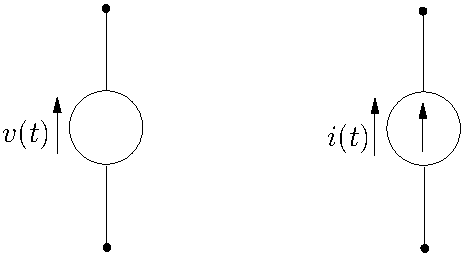
\includegraphics[width=6cm]{sources}
\caption{Sources de tension et de courant}
\label{fig:sources}
\end{center}
\end{figure}
\item{\em Les sources de courant} représentées par le symbole de
la figure \ref{fig:sources} sont des dip{ô}les définis par le
courant $i(t)$ qu'ils débitent indépendamment de la tension à
leurs bornes. 
\end{enumerate} 
\end{description}
Il est important de bien comprendre que les impédances et les sources sont des modèles conceptuels idéaux qui n'ont pas d'existence physique. Les différents éléments dont sont constitués les circuits électriques réels comme par exemple des bobines, des condensateurs ou des batteries sont en pratique modélisés par des assemblages appropriés d'inductances et de sources. Par exemple une source de tension ou de courant est toujours modélisée avec son inévitable résistance interne, comme indiqué sur la fig.~\ref{fig:resint}.

\begin{figure}[t]
\begin{center}
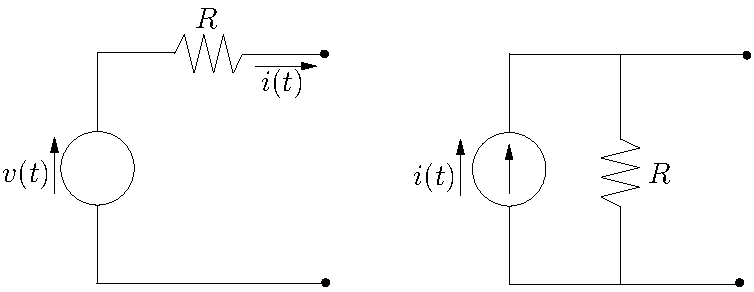
\includegraphics[height=4cm]{resint}
\caption{Sources avec résistances internes}
\label{fig:resint}
\end{center}
\end{figure}


\section{Equivalence entre systèmes ouverts et fermés}

Nous avons vu un système électrique comme ``ouvert'', c'est-à-dire muni de variables d'entrées et de sortie, qui sont des courants ou des tensions. L'ajout de sources permet toutefois de considérer un système fermé équivalent. Par exemple un dipôle dont la tension $v(t)$ est l'entrée, peut être fermé par une source de tension variable qui délivre précisément la tension $v(t)$ (voir fig.~\ref{fig:equivouvertferme}). Il est quelquefois commode pour l'analyse de se ramener à un graphe fermé.


\begin{figure}[htbp]
\begin{center}
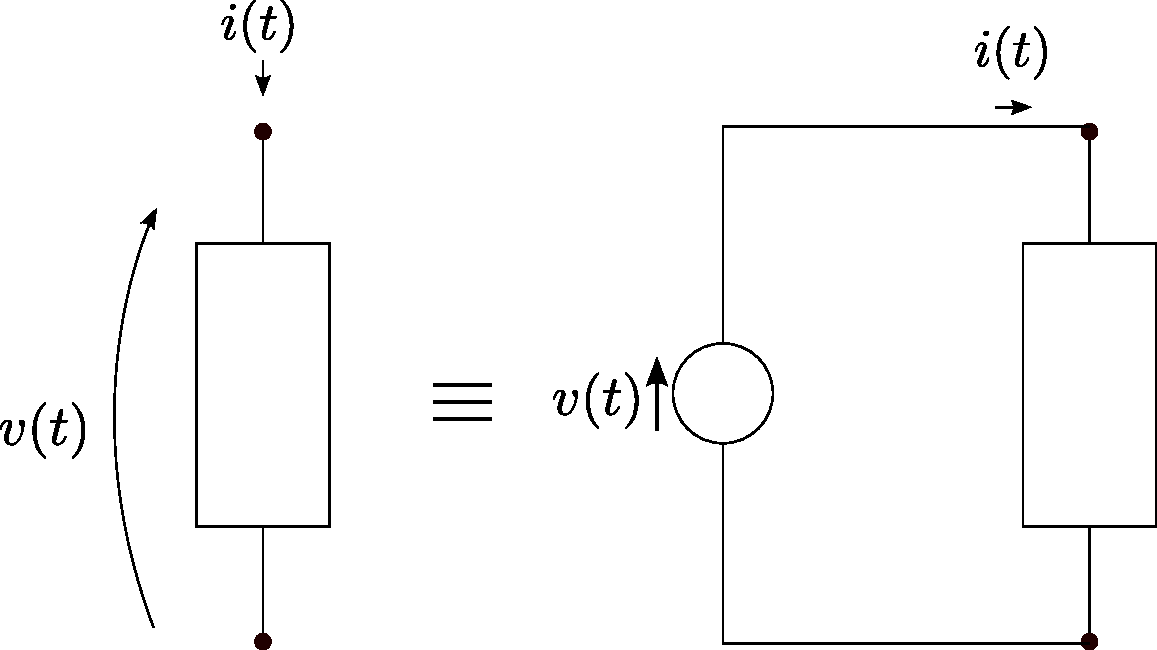
\includegraphics[width=6cm]{equivouvertferme}
\caption{Equivalence entre un circuit ouvert et un circuit fermé: le cas d'un dipôle dont l'entrée est la tension, et la sortie le courant}
\label{fig:equivouvertferme}
\end{center}
\end{figure}

Si le dipôle est conçu pour fournir de l'énergie à l'extérieur ($v(t) i(t) >0$), alors on peut également fermer le circuit par la charge supposée absorber l'énergie, qu'on modélise souvent comme une (grande) résistance de charge. Ceci est une restriction, car la charge pourrait être autre chose qu'une résistance. Par exemple un moteur est plutôt de nature inductive.

\section{Réseaux électriques et mise en équation du modèle d'état}

Les systèmes électriques complexes sont généralement créés par l'interconnection en réseau d'un nombre fini de systèmes élémentaires. Dans ce chapitre nous considérons les réseaux formés de  dipôles élémentaires (impédances et sources). Il est clair qu'un tel
réseau a une structure de graphe dont les branches sont formées
par les dip{ô}les. Un exemple de réseau
et de graphe  associé est donné à la figure
\ref{fig:exemplereseau} qui représente un pont d'impédances. Les flèches sur le graphe indiquent le sens conventionnel choisi pour le courant dans chacune des branches. 
\begin{figure}[t]
\begin{center}
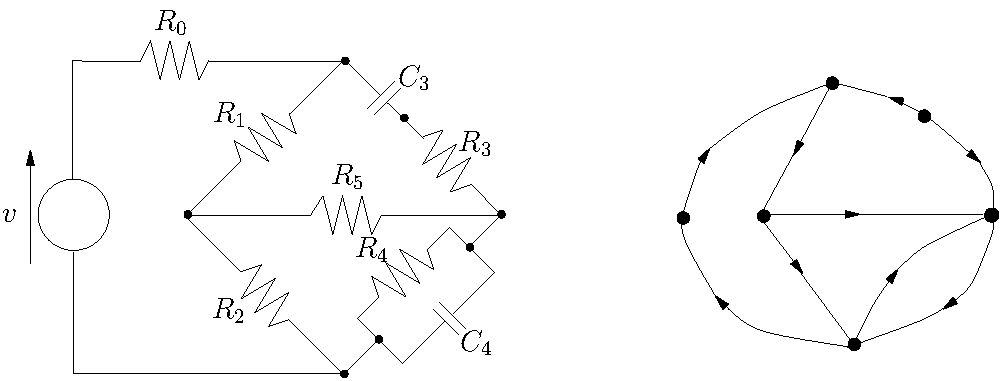
\includegraphics[height=45mm]{exemplereseau}
\caption{Pont d'impédances}
\label{fig:exemplereseau}
\end{center}
\end{figure}
Nous considérons des réseaux électriques fermés (au moyen de sources de tension et/ou de courant, voire avec des résistances de charge) {\bf connexes} 
comportant $N$ noeuds et $M$ branches. 
% et qui satisfont l'hypothèse
%suivante (voir figure \ref{fig:resint}) : {\em toutes les sources de tension sont incorporées dans
%une branche avec une résistance interne en série, toutes les sources de
%courant possèdent une résistance interne en parallèle}.  
Un graphe est connexe lorsqu'il existe toujours un chemin du graphe reliant deux
noeuds quelconques.

Définissons deux notions utiles par la suite : les
mailles et les coupes d'un réseau électrique.
\begin{description}
\item Une {\em maille} est un cycle, c'est-à-dire un chemin ``fermé" sans répétition de noeud.
\item Une {\em coupe} est ensemble  de branches dont
l'extraction partage un réseau connexe en au moins deux sous-réseaux connexes séparés.
\end{description}

L'établissement du modèle d'état d'un réseau électrique est
basé sur les lois de Kirchhoff qui s'énoncent comme suit :
\begin{itemize}
\item Loi de Kirchhoff des courants : la somme algébrique des
courants dans les branches incidentes à un noeud est nulle.
\item Loi de Kirchhoff des tensions : la somme algébrique des
tensions dans une maille est nulle.
\end{itemize}


Si le graphe est fermé, la somme des équations de Kirchhoff de courant sur tous les $N$ noeuds donne l'égalité triviale $0=0$, car chaque courant intervient deux fois avec un signe opposé. Il y a $N-1$ équations de Kirchhoff indépendantes sur les courants. Pour toute coupe, on trouve également que la somme des courants sur les branches de la coupe est nulle, ce qui est obtenu en sommant les équations de Kirchhoff des courants sur tous les noeuds d'un côté de la coupe.

Pour trouver le nombre d'équations indépendantes de Kirchhoff sur les mailles dans un réseau fermé, considérons un arbre sous-tendant du graphe, c'est-à-dire un sous-graphe connexe, sans maille et incident à tous les noeuds. Un tel arbre a $N-1$ arêtes. Chaque branche du réseau ajoutée à cet arbre  créée une et une seule nouvelle maille indépendante. On peut ainsi créer $M-N+1$ équations de maille qui se trouvent être indépendantes.


Les variables d'état d'un réseau sont les courants dans
certaines inductances et les tensions aux bornes de certaines
capacités.   Pour établir le modèle d'état d'un réseau, il suffit
de procéder comme suit :
\begin{enumerate}
\item Ecrire $N-1$ équations de Kirchhoff  pour les courants.
\item Ecrire $M-N+1$ équations de Kirchhoff linéairement
indépendan\-tes pour les tensions.
\item Ecrire les lois de définition des impédances correspondant
aux  tensions ou aux courants intervenant dans les équations de
Kirchhoff 
\item Eliminer les tensions et les courants redondants.
\end{enumerate}

Il est à noter que si un circuit comporte plusieurs branches successives formant un dipôle composé de plusieurs dipôles élémentaires en série, les lois de Kirchhoff de courant sur les noeuds intermédiaires seront triviales. De même les équations de Kirchhoff de maille ne feront intervenir que la tension totale du dipôle, et non les tensions élémentaires isolément.
En ce qui concerne l'écriture des équations de Kirchhoff, on peut donc compter ce dipôle composé comme  créant une seule branche et deux noeuds.


Si le réseau contient une maille de capacités, il est clair que la tension aux bornes d'une de ces capacité peut être écrite comme la somme (signée) des autres, créant une relation linéaire en variables d'état. A contrario, lorsque le réseau ne contient pas de mailles de capacités, toutes
les tensions aux bornes des capacités sont des variables d'état indépendantes.
De même, toute coupe d'inductances impose une relation linéaire entre les courants qui les traversent, puisque leur somme (signée) est nulle. Un de ces courants n'est donc pas pris comme variable d'état indépendante. A contrario, lorsqu'un réseau ne contient pas de coupes d'inductances,
tous les courants dans les inductances sont des variables d'état indépendantes. 
%Dans ce
%cas, on peut d'emblée réduire le nombre $M$ de branches et le nombre $N$
%de noeuds en convenant qu'une branche peut être définie comme un
%ensemble de dipôles placés en série et comportant au plus une capacité
%ou une inductance.
\begin{exemple}{\bf \em Circuit redresseur avec filtre LC}

\begin{figure}[htbp]
\begin{center}
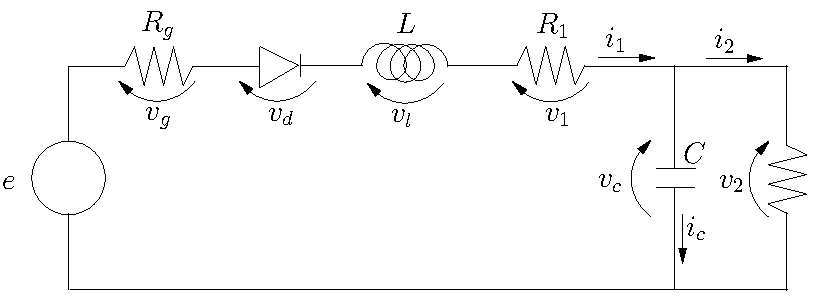
\includegraphics[height=4cm]{redresseur}
\caption{Circuit redresseur}
\label{fig:redresseur}
\end{center}
\end{figure}
La figure \ref{fig:redresseur} représente un circuit
redresseur à diode avec un filtre formé d'une capacité et d'une
inductance. La diode est une résistance nonlinéaire dont la caractéristique courant-tension s'exprime comme suit :
\eqnn
i = i_0[e^{\frac{v}{\alpha}} -1]
\eeqnn
où $\alpha$ est une constante proportionnelle à la température
et inversement proportionnelle à la charge de l'électron, tandis
que $i_0$ désigne le courant de fuite de la diode.  Il est clair que
ce circuit ne contient ni maille de capacités ni coupe
d'inductances.  Donc son modèle d'état comportera deux variables
d'état : la tension $v_c$ aux bornes de la capacité et le courant
$i_1$ dans l'inductance.

Le circuit comporte $N=6$ noeuds et $M=7$ branches. Toutefois on peut par commodité regrouper les dipôles en série en une seule branche, ce qui nous laisse $N=2$ noeuds et $M=3$ branches.  Pour établir le modèle d'état du système, on écrit $N-1 = 1$
équation de Kirchhoff pour les courants : 
\eqnn
i_c - i_1 + i_2 = 0,
\eeqnn
et $M-N+1 =2$ équations de Kirhhoff pour les tensions :
\begin{equation} \begin{split}
&v_c - v_2 = 0,\\
&v_g +v_d +v_\ell +v_1 +v_c -e = 0.
\end{split} \end{equation}
Ces équations sont complétées par les équations de
définition des divers éléments du circuit :
\begin{equation*} \begin{split}
v_g &= R_gi_1, \\
v_d &= \alpha \ln \frac{i_0+i_1}{i_0},\\
v_\ell &= L \frac{di_1}{dt},\\
i_c &= C \frac{dv_c}{dt}, \\
v_1 &= R_1i_1,\\
v_2 &=R_2i_2.
\end{split} \end{equation*}
En éliminant les 7 variables $i_2,i_c, v_g, v_d, v_\ell, v_1, v_2$
entre ces 9 équations, on obtient aisément les deux équations
suivantes~:
\eqnn
&&R_gi_1 + \alpha \ln \frac{i_0+i_1}{i_0} + L \frac{di_1}{dt} + R_1i_1
+ v_c - e = 0,\\
&&C\frac{dv_c}{dt} - i_1 + \frac{v_c}{R_2} = 0.
\eeqnn
En définissant les variables d'état et d'entrée comme suit :
\e
x_1 = i_1, \;\;\; x_2= v_c, \;\;\; u = e,
\ee
on obtient finalement les équations d'état :
\begin{equation*} \begin{split}
\dot x_1 &= -\frac{R_1+R_g}{L} x_1 - \frac{\alpha}{L} \ln
\left(\frac{i_0+x_1}{i_0} \right) - \frac{1}{L} x_2 + \frac{1}{L} u,\\
\dot x_2 &= \frac{1}{C} x_1 - \frac{1}{R_2C} x_2 
\end{split} \end{equation*}
\cqfd

\end{exemple}

Lorsque le réseau contient des mailles de capacités ou des coupes
d'inductances, on cherche une forêt (sous-graphe sans maille) de capacités de taille maximale, et une non-coupe d'inductances 
de taille maximale. Le nombre de capacités et d'inductances ainsi sélectionnées est le nombre de variables d'état indépendantes.

%On introduit les définitions
%suivantes :
%\begin{description}
%\item {\em Arbre} : un arbre est un sous-réseau connexe qui contient
%tous les noeuds du réseau mais ne comporte aucune maille (tous les
%arbres d'un réseau ont le même nombre de branches : $N-1$).
%\item {\em Co-arbre}: un co-arbre est le sous réseau
%complémentaire d'un arbre (tous les co-arbres d'un réseau ont le
%même nombre de branches: $M-N+1$).
%\end{description}
%Le nombre de
%variables d'état peut alors être déterminé par la règle suivante :

On peut montrer aisément que ceci revient trouver un arbre qui contienne  le plus grand nombre possible de capacités, tel que le co-arbre (i.e. le sous-réseau complémentaire de l'arbre) contienne le plus grand nombre possible d'inductances.Le nombre de variables d'état indépendantes est alors la somme du nombre de
capacités de l'arbre et du nombre d'inductances du co-arbre.

%L'intuition de cette règle peut se comprendre en observant que les capacités contenues dans un arbre (par définition sans maille) déterminent toutes des variables d'états linéairement indépendantes. On cherchera donc un arbre qui en contiennent le plus grand nombre. De même un coarbre ne contient pas de coupe du réseau. Il est donc avantageux d'y placer un nombre maximal d'inductances, dont les
%courants formeront des variables d'état linéairement indépendantes. Un peu d'algèbre linéaire montre qu'on obtient ainsi un ensemble complet et non redondant de variables d'état. 


\section{Les systèmes électromécaniques} 

Un système mécanique pourrait être défini similairement à un système électrique, dont les bornes 
sont soumises,  non pas à des courants et des voltages, mais à des forces $F_i$ et des vitesses $v_i=\dot{q}_i$ (à ne pas confondre avec le symbole de tension).  La translation de toutes les vitesses $v_i(t)$ vers $v_i(t)+v$ ne modifie pas le comportement du système, par relativité galiléenne. La somme des forces $\sum_{i} F_i(t)$ est en générale nulle à tout moment dans les systèmes mécaniques de l'ingénieur. L'énergie mécanique transmise au système est dans ces conditions univoquement définie comme $\sum_i F_i(t) v_i(t)$.
Certaines forces ou vitesses sont choisies comme entrées, et d'autres comme sorties. Un exemple de dipôle mécanique est la combinaison de deux forces opposées $F_1(t)+F_2(t)=0$ s'appliquant à des points différents, qui peut être résumé à un couple $T$ et une vitesse angulaire $\omega$ (voir Chapitre 2).

Un système électromécanique est bien sûr défini comme une boîte noire dont certaines variables sont de nature électrique et d'autres de nature mécanique (voir fig.~\ref{fig:systemelectromec}).


\begin{figure}[t]
\begin{center}
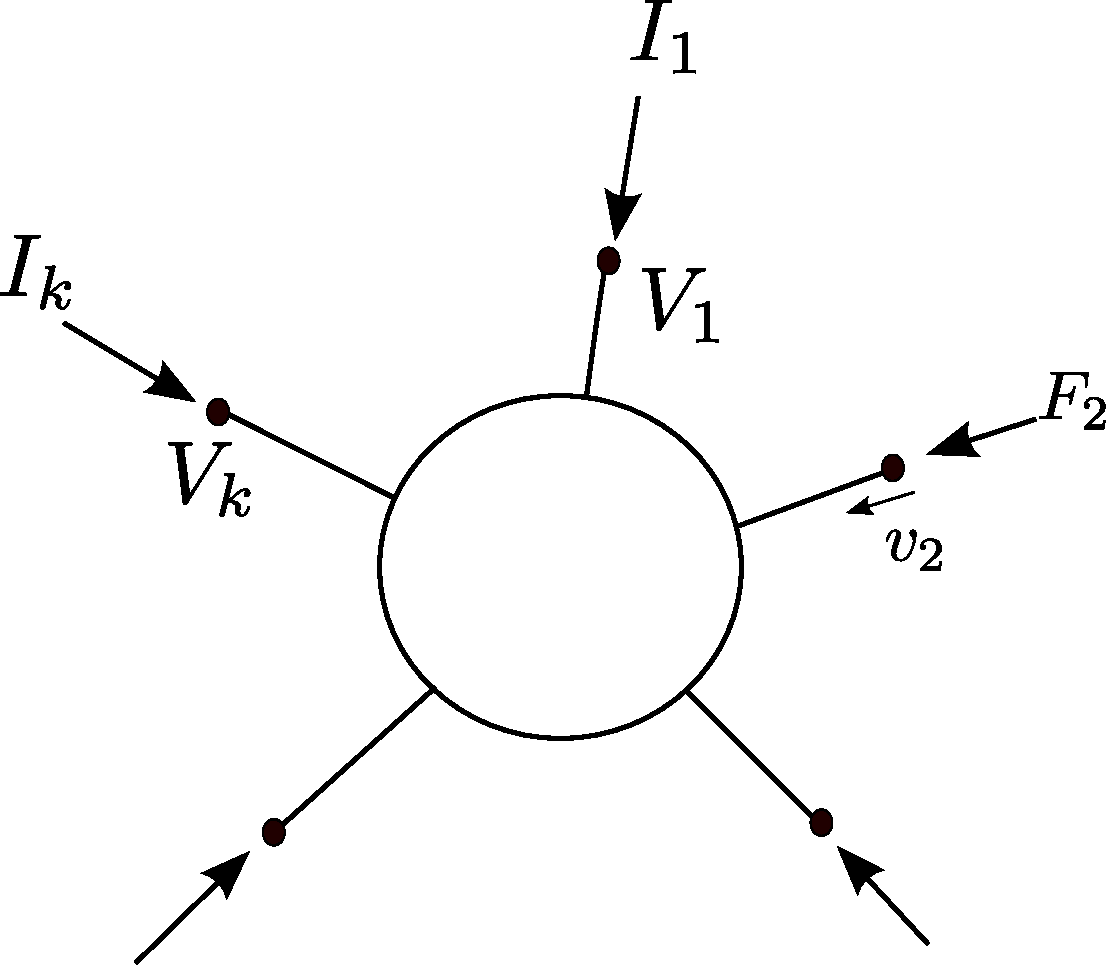
\includegraphics[width=7cm]{systemelectromec}
\caption{Système électromécanique}
\label{fig:systemelectromec}
\end{center}
\end{figure}

Par exemple un quadrupôle électromécanique dont les variables sont $v(t)$, $i(t)$, $T(t)$,  $\omega(t)$ peut modéliser un générateur si $T\omega<0, vi>0$ (énergie électrique convertie en énergie mécanique) ou un moteur si $T\omega>0, vi<0$ (énergie mécanique convertie en énergie électrique).


\begin{figure}[t]
\begin{center}
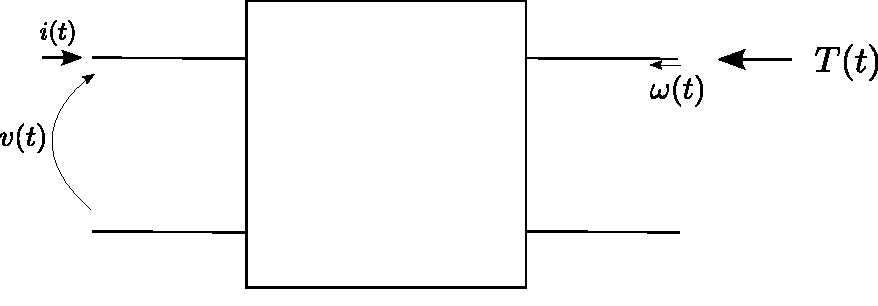
\includegraphics[width=7cm]{quadrupelectromec}
\caption{Quadrupôle électromécanique}
\label{fig:quadrupelectromec}
\end{center}
\end{figure}


Concrètement, un système électromécanique se présente souvent comme un système
mécanique articulé (à $p$ degrés de liberté) qui peut être
construit partiellement dans un matériau magnétique et dont
certains corps portent un ou plusieurs circuits électriques inductifs (bobines,
enroulements, etc.). Les équations constitutives d'un système
électromécanique comportent dès lors une partie mécanique et
une partie électrique.

Les deux section suivantes expliquent, via quelques rappels d'électromagnétisme, comment les variables électromagnétiques (charges, flux, courants, tensions) et mécaniques (positions, vitesses, forces généralisées) peuvent interagir.

\section{Influence d'un mouvement mécanique sur les grandeurs électriques} 

La loi de Faraday $E_i=\frac{d\phi_i}{dt}$ décrit la force électromotrice (tension) subie par une inductance traversée par un flux magnétique $\phi_i$. Jusqu'ici on a supposé que ce flux était créé uniquement par le courant $I_i$ qui la traverse (auto-inductance). Pour une relation linéaire $\phi_i=L_iI_i$, on obtient la loi constitutive $V_i=L_i \dot{I}_i$.

En réalité chaque courant $I_j$ génère un champ magnétique et donc un flux dans l'inductance $i$. Ce flux dépend de $I_j$, mais aussi de la position relative des conducteurs qui portent ces courants, éventuellement variable dans le temps à cause d'un mouvement mécanique des pièces qui supportent les conducteurs.
Généralement seuls les courants qui traversent une inductance génèrent un champ magnétique non négligeable. Si $\phi_i$ dépend linéairement de chaque $I_j$, on peut écrire
\begin{equation}
\phi_i=\sum_j L_{ij} I_j,
\label{eq:PhiLI}
\end{equation}
où $L_{ii}$ est l'auto-inductance. En notation matricielle cela donne
\begin{equation}
\Phi=L(q) I,
\label{eq:PhiLI2}
\end{equation}
où $L(q)$ est une matrice symétrique d'inductance dépendant des positions généralisées $q$ de la partie mécanique. En combinant ceci avec l'équation de Faraday pour chaque inductance, on arrive aux équations d'état
\begin{equation}
E=\sum_k \frac{\partial L}{\partial q_k} \dot{q}_k I + L\dot{I},
\label{eq:VqI}
\end{equation}
qui mêlent positions, vitesses, courants et tensions.

La composante électrique des systèmes électromécaniques visités dans ce chapitre est souvent élémentaire, réduite à un ensemble d'inductances, chacune en série avec une résistance représentant l'inévitable résistance interne ou bien une résistance de charge, qui représente la consommation utile d'énergie électrique éventuellement générée par le système (voir fig.~\ref{fig:circel}). Dans ce cas, les tensions aux bornes des circuits s'écrivent de manière matricielle
\eqn
V = RI + E \label{ELECM}
\eeqn
où $R$ est la matrice $\mbox{diag}\{R_i, i = 1,m\}$ et les
vecteurs $V,I$ et $E$ sont définis comme suit :
\begin{equation*} \begin{split}
V^T &= (v_1, v_2, \ldots, v_m),\\
I^T &= (I_1, I_2, \ldots, I_m),\\
E^T &= (E_1, E_2, \ldots, E_m).
\end{split} \end{equation*}
\begin{figure}[t]
\begin{center}
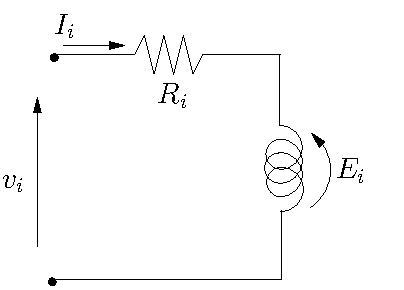
\includegraphics[height=4cm]{circel}
\caption{Circuit élémentaire}
\label{fig:circel}
\end{center}
\end{figure}



\section{Création d'un mouvement mécanique par les grandeurs électromagnétiques} 

Un champ magnétique exerce une force dite de Lorentz sur chaque porteur de charge en mouvement. En intégrant cette force sur tous les porteurs de charge mis en mouvement par un courant électrique dans un conducteur on obtient une force macroscopique, dite de Laplace.  

%Pour peu que ce conducteur appartienne à une boucle rectangulaire de dimension $l \times z$ et soit mobile dans la direction de $z$ (voir Fig.~\ref{fig:laplace}, on constate que cette force de Laplace est aussi proportionnelle à $\frac{\partial \phi}{\partial z}I$,
%où $\phi$ est le flux créé par $B$ dans la boucle traversée par le courant $I$. 

%\begin{figure}[t]
%\begin{center}
%\includegraphics[width=7cm]{laplace}
%\caption{Force de Laplace sur un conducteur mobile posé sur deux rails conducteur}
%\label{fig:laplace}
%\end{center}
%\end{figure}



En général, on peut montrer que la force de Laplace sur la coordonnée $q_k$ est 
\begin{equation}
F_k=\frac{1}{2}\sum_i \frac{\partial \phi_i}{\partial q_k}  I_i = \frac{1}{2} I^T \frac{\partial L}{\partial q_k} I,
\label{eq:Lorentz}
\end{equation}
la dernière égalité concernant les inductances linéaires. Dans ce dernier cas, on peut déduire directement l'expression $F_k$  en supposant que la force dérive d'une énergie potentielle contenue dans les inductances qui génèrent les champs magnétiques, exprimée par $\frac{1}{2} I^T L(q_k) I$.




%\begin{description}
%\item{\em Equations mécaniques}.  Les équations
%de la partie mécanique prennent la forme générale que nous avons
%obtenue au chapitre 2.
%\eqn
%M(q) \ddot q + F(q, \dot q) = G_{em}(q) u_{em} + G_a(q)u_a.
%\label{EMECA}
%\eeqn
%Dans cette équation, $u_{em}$ représente les forces
%généralisées d'origine électromagnétique (équation de Lorentz)
%tandis que $u_a$ désigne les autres forces généralisées qui
%s'appliquent éventuellement au système. $q$ est un vecteur de dimension $p$.
%\item {\em Equations électriques}.  Chacun des circuits électriques
%du système peut être conceptualisé par le circuit
%élémentaire représenté sur la fig \ref{fig:circel} où
%$R_i$ représente la résistance propre du circuit et $E_i$
%représente la tension induite par les variations de flux magnétiques produits par les différents
%circuits (y compris l'auto-induction) et par le mouvement du système
%(loi d'induction électromagnétique ou loi de Lenz). 
%\begin{figure}[t]
%\begin{center}
%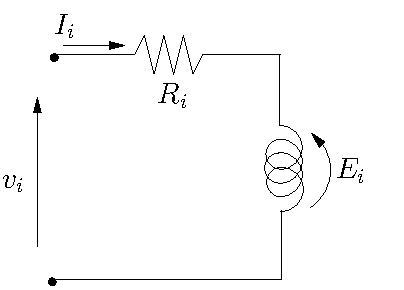
\includegraphics[height=4cm]{circel}
%\caption{Circuit élémentaire}
%\label{fig:circel}
%\end{center}
%\end{figure}
%Si l'on
%suppose que le système comporte $m$ circuits, on obtient
%un ensemble d'équations de Kirchhoff de la forme
%\eqnn
%R_i I_i +E_i = v_i, \;\;\;   i = 1, \ldots, m.
%\eeqnn
%Dans ces équations, $v_i$ représente la tension aux bornes du
%dip{ô}le équivalent du réseau connecté au circuit.  Le plus
%souvent, il s'agit simplement soit d'une source de tension ou de
%courant, soit d'une impédance de charge.  L'ensemble des équations
%électriques peut aussi s'écrire sous forme matricielle
%\eqn
%V = RI + E \label{ELECM}
%\eeqn
%où $R$ est la matrice $\mbox{diag}\{R_i, i = 1,m\}$ et les
%vecteurs $V,I$ et $E$ sont définis comme suit :
%\begin{equation*} \begin{split}
%V^T &= (v_1, v_2, \ldots, v_m),\\
%I^T &= (I_1, I_2, \ldots, I_m),\\
%E^T &= (E_1, E_2, \ldots, E_m).
%\end{split} \end{equation*}
%\end{description}
%La mise en équation complète du modèle d'état d'un système
%électro\-mécanique particulier requiert l'explicitation des
%{\em couplages} entre la partie mécanique (\ref{EMECA}) et
%la partie électrique (\ref{ELECM}), c'est à dire l'expression des
%forces généralisées électromagnétiques $u_{em}$ d'une part et
%des tensions induites $E$ d'autre part comme des
%fonctions des coordonnées mécaniques $q, \dot q$ et des courants
%électriques $I$~:
%\eqnn
%u_{em}(q, \dot q, I), \hspace{1cm} E(q,\dot q, I). 
%\eeqnn 
%Chacune des tensions $E_i$ peut se décomposer comme
%suit~:
%\eqn \label{ei}
%E_i = \sum^m_{j=1} e_{ji} 
%\eeqn
%où $e_{ji}$ représente la tension induite par le circuit $j$ sur le
%circuit $i$ (en particulier, $e_{ii}$ représente l'auto-induction
%du circuit $i$). Par application de la loi de Faraday, chacune de ces tensions
%s'exprime comme suit :
%\eqnn
%e_{ji} = \frac{d\phi_{ji}}{dt}
%\eeqnn
%où $\phi_{ji}$ est le flux induit par le circuit $j$ sur le circuit
%$i$.
%Le flux $\phi_{ji}$ varie en fonction du courant $I_j$ dans le
%circuit inducteur et de la position $q$ du système :
%\eqnn
%\phi_{ji} = \varphi_{ji}(q, I_j).
%\eeqnn
%On en déduit que la tension $e_{ji}$ s'écrit :
%\eqn \label{eij}
%e_{ji} = \frac{\partial \varphi_{ji}}{\partial q} \dot q +
%\frac{\partial \varphi_{ji}}{\partial I_j} \dot I_j.
%\eeqn
%D'autre part, la composante d'indice $k$ du vecteur
%des forces généralisées $u_{em}$ s'écrit 
%\eqn
%u_{em(k)} = \frac{1}{2} \sum^m_{i=1} \sum^m_{j=1} \frac{\partial
%\varphi_{ji}}{\partial q_k} I_i. \label{uem}
%\eeqn
%Finalement, en combinant les équations (\ref{EMECA}),(\ref{ELECM}),
%(\ref{ei}), (\ref{eij}), (\ref{uem}), on obtient un modèle d'état
%comportant $2p + m$ variables d'état $q, \dot q, I$.

\vspace{2mm}
\begin{exemple}{\bf \em  Un système électromécanique de positionnement.} 
 
Le schéma de principe d'un électro-aimant utilisé pour un positionnement de précision est indiqué à la figure
\ref{fig:relaisem}.
\begin{figure}[htbp]
\begin{center}
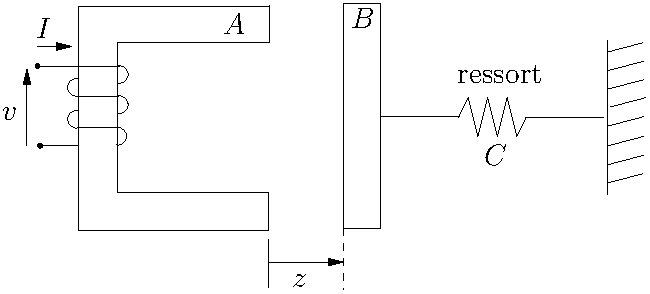
\includegraphics[height=4cm]{relaisem}
\caption{Système électro-mécanique de positionnement}
\label{fig:relaisem}
\end{center}
\end{figure}
L'électro-aimant $A$ est muni d'une bobine
inductrice dans laquelle circule un courant inducteur $I$.  La pièce
métallique $B$ est mobile et soumise à une force de rappel
linéaire par le ressort $C$.

Le flux magnétique varie proportionnellement au courant $I$
et inversément proportionnellement à la distance $z$ dans
l'entrefer : 
\eqnn
\phi (I,z) = \frac{\alpha I}{1+\beta z}.
\eeqnn
Ceci est une instance de la loi d'Ohm magnétique (ou loi d'Hopkinson), qui exprime le flux magnétique (équivalent du courant, flux de charges électriques) comme le ratio entre la force magnétomotrice (proportionnelle au courant) et la réluctance (résistance du matériau au flux magnétique), qui est proportionnelle à la longueur du circuit.

La tension induite dans le circuit s'écrit donc :
\eqnn
e &=& \frac{d\phi}{dt} = \frac{\partial \phi}{\partial I}
\frac{dI}{dt} + \frac{\partial \phi}{\partial z} \frac{dz}{dt}\\
&=&\frac{\alpha}{1+\beta z} \frac{dI}{dt} - \frac{\alpha \beta
I}{(1+\beta z)^2} \frac{dz}{dt}.
\eeqnn
La force d'origine électromagnétique s'exer\c cant sur la pièce
mobile s'écrit :
\eqnn
F_{em} = \frac{1}{2} I \frac{\partial \phi}{\partial z} = -
\frac{\alpha \beta}{2} \left(\frac{I}{1+\beta z}\right )^2.
\eeqnn
En accord avec l'intuition physique, on observe que cette force tend
à rapprocher la pièce $B$ de l'électro-aimant quel que soit le
sens du courant $I$.

On peut alors écrire les équations dynamiques du
système. \\

\begin{itemize}
\item{\em Equation mécanique}
\begin{eqnarray}
m \ddot z &=& k(z_o - z) + F_{em}\\
&=& k(z_o - z) - \frac{\alpha \beta}{2} \left (\frac{I}{1+\beta z}
\right )^2
\end{eqnarray}
où $m$ désigne la masse de la pièce $B$, $k$ la
constante de rappel du ressort et $z_o$ la position du ressort au repos.\\
\item{\em Equation électrique}
\begin{eqnarray}
V&=& RI + e\\
  &=& RI + \frac{\alpha}{1+\beta z} \dot I - \frac{\alpha \beta I}{(1+
\beta z)^2} \dot z 
\end{eqnarray}
où $R$ désigne la résistance du circuit électrique.
\end{itemize}

En introduisant les définitions suivantes des variables
d'état : 
\eqnn
x_1 = z, \;\;\; x_2 = \dot z, \;\;\; x_3 = I
\eeqnn
et de la variable d'entrée :
\eqnn
u = V,
\eeqnn
on obtient finalement le modèle d'état du système :
\begin{eqnarray}
\dot x_1 &=& x_2,\\
\dot x_2 &=& \frac{k}{m}(z_o - x_1) - \frac{\alpha \beta}{2m} \left
(\frac{x_3}{1+ \beta x_1} \right )^2,\\
\dot x_3 &=& \frac{\beta x_2 x_3}{1+\beta x_1} - \frac{R}{\alpha}(1+
\beta x_1) x_3 + \frac{1 + \beta x_1}{\alpha} u.
\end{eqnarray}
\cqfd

\end{exemple}

\section{Rotating electric machines}

The rotating electric machines constitute a particular category of electromechanical systems formed by two bodies. The first one, called {\em rotor}, is in rotation around an axe whose position is fixed to the second one, called {\em stator}. These two pieces are provided with different \blue {field windings} whose utility is to realise electromechanical conversions of which the machines are the centre. 

When the stator itself is fixed to the inertial landmark, an electrical machine has only one mechanical degree of freedom : the rotor’s rotation angle, written $\theta$. The mechanical part of the system shrinks therefore to a scalar equation of the form : 

\eqn \label{meca}
J \ddot \theta + h(\dot \theta) = T_{em}+ T_a 
\eeqn
where $h(\dot \theta)$ represents the friction torque, $T_{em}$ the electromagnetical torque and $T_a$ all the other external torques applied to the rotor. 

On the other hand, the electrical part of the dynamic has the general form (\ref{ELECM}) :
\eqnn
V = RI + E. 
\eeqnn

In most running machines, when the magnetical saturation effects are negligible (or neglected), it is possible to present the flows $\phi_{ij}$ by an expression of the form : 

\eqnn
\phi_{ij} = L_{ij}(\theta)I_i
\eeqnn
which is linear to the inductor current $I_i$ but that depends on the angular position $\theta$ of the rotor, following a law $L_{ij}(\theta)$ usually periodic. The inductance matrix (symmetrical) is defined as : 

\eqnn
L(\theta) \triangleq [L_{ij}(\theta)]
\eeqnn
and its derivative to $\theta$ is : 
\eqnn
K(\theta) \triangleq \frac{\partial L(\theta)}{\partial \theta}.
\eeqnn
Then, the use of the theory that was introduced in the last sections leads to general equations of electromechanical coupling, whose form is the following: 
\begin{align}
E &= L(\theta)\frac{dI}{dt} + \frac{d\theta}{dt}K(\theta)I, \label{coup1}\\
T_{em} &= \frac{1}{2}I^TK(\theta)I. \label{coup2}
\end{align}
By combining the equations (\ref{meca}),(\ref{ELECM}),(\ref{coup1}) and (\ref{coup2}) we get the general model of the electrical machines~: 
\begin{equation*} \begin{split}
L(\theta)\dot I &= - \omega K(\theta) I - RI + V, \\
\dot \theta &= \omega, \\
J \dot \omega &= \frac{1}{2} I^TK(\theta)I - h(\omega) + T_a.
\end{split} \end{equation*}
It is this general model that is on the basis of the particular models establishment in the applications. Often, but it not a standard, the voltage vector $V$ or the torque $T_a$ are parameterized by  well selected entrance variables that represent the external influence on the machine’s behaviour. Here is an example. Other examples are provided in the exercises. 

\begin{exemple}{\bf \em Elementary machine with two windings}

Let’s consider an electrical machine whose rotor and stator are concentric cylinders with a winding on the stator and another on the rotor ( Fig.~\ref{fig:rotorstator}). The statorical and rotorical auto-inductances $L_s$ and $L_r$ are constants. The mutual inductance $L_{sr}$ is a cosinusoidal periodical function of angle $\theta$  

\eqnn
L_{sr}(\theta) = L_o \cos \theta.
\eeqnn

Matrices $L(\theta)$ and $K(\theta)$ are written as follows:

\eqnn
L(\theta) =   \bma{cc} L_s & L_o \cos \theta\\ L_o \cos \theta & L_r \ema
\;\;\;\;  K(\theta) = \bma{cc} 0 & -L_o \sin \theta\\ -L_o \sin \theta & 0
\ema.
\eeqnn
Vectors of current and induced tensions are noted : 
\eqnn
I = \bma{c} I_s \\ I_r \ema \;\;\;\; E = \bma{c} e_s \\ e_r \ema.
\eeqnn
Electromechanical coupling equations (\ref{coup1}), (\ref{coup2})  particularize themselves by:
\begin{equation*} \begin{split}
e_s &= L_s \dot I_s + L_o \cos\theta \dot I_r - \dot \theta L_o \sin \theta
I_r, \\ 
e_r &= L_r \dot I_r + L_o \cos\theta \dot I_s - \dot \theta L_o \sin
\theta I_s, \\
T_{em} &= -L_o \sin \theta I_sI_r.
\end{split} \end{equation*}
The rotorical circuit is being supplied by a constant current source $I_r$. Such a machine can be used either as a generator (that transforms the mechanical power provided by the external torque $T_a$ in electrical power delivered by the statoric electromotive power $e_s$), or as an engine  (that transforms the electrical power delivered to the stator by the source $v_s$  in a mechanical power delivered by the electromagnetical torque $T_{em}$). 

\begin{figure}[htbp]
\begin{center}
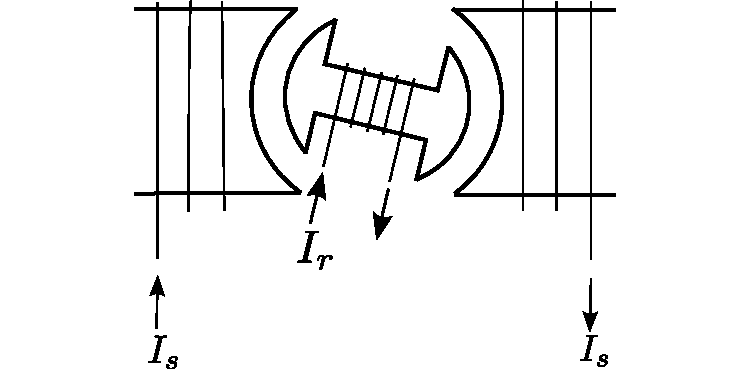
\includegraphics[height=5cm]{rotorstator}
\caption{Elementary machine with two windings}
\label{fig:rotorstator}
\end{center}
\end{figure}

The system has three state variables :
\begin{equation*} \begin{split}
x_1 &= I_s, \\
x_2 &= \theta, \\
x_3 &= \dot \theta,
\end{split} \end{equation*}
and two input variables :
\begin{equation*} \begin{split}
u_1 &= v_s, \\
u_2 &= T_a.
\end{split} \end{equation*}
The state-spaced model of the system is noted as follows: 
\begin{align*}
L_s\dot x_1 &= L_oI_rx_3 \sin x_2 - R_s x_1 + u_1, \\
\dot x_2 &= x_3, \\
J\dot x_3 &= -h(x_3) - L_oI_rx_1 \sin x_2 + u_2.
\end{align*}

In the case of generator mode, we can also close the electrical part of the circuit with a resistance of charge $R_L$, we can then set $u_1=R_L x$ and we obtain a state-spaced model with only one input $u_2=T_a$.

\cqfd



\end{exemple}

\section{Direct current machines}
\markboth{{\hspace*{5mm}\bf Chapitre 3} \hfill Electrcical systems}{{ \bf Sec. \thesection}
\hfill Direct current machines\hspace*{5mm}} 


Direct current machines (fig.
\ref{fig:machineDC}) generally include a stator winding and a rotor one.  
\begin{figure}[t]
\begin{center}
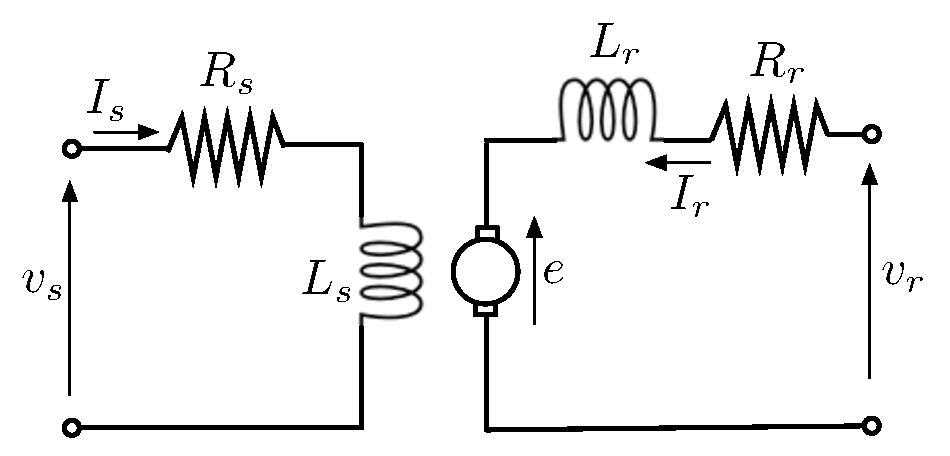
\includegraphics[height=4cm]{machineDC}
\caption{Direct current machines}
\label{fig:machineDC}
\end{center}
\end{figure}

The stator winding is the inductive circuit whose current is noted  by $I_s$. The rotor winding is the \blue {induced circuit} whose current is written by $I_r$. 

So a direct current machine (DC machine) seems similar to the elementary two-winding machine we studied in the previous section. However, there is a fundamental difference : a DC machine is designed with a 
\blue {commutation} system whose effect is to modify the electromechanical coupling. A detailed description of this commutation effect on the coupling equations is beyond the scope of this book.  So we restrict ourselves to give the results. When the effect of magnetic saturation are negligible and when the commutation  
doesn't generate significant non-linearities, the equations  of electromechanical coupling  of a DC machine are witten  as the following multilinear form :
 
\begin{equation*} \begin{split}
&e_s = L_s \frac{dI_s}{dt}, \\[2mm]
&e_r = L_r \frac{dI_r}{dt} + \frac{d\theta}{dt}K_eI_s, \\[2mm]
&T_{em} = K_mI_rI_s.
\end{split} \end{equation*}
Let's notice the the \blue {resemblance, but not the similarity},
of those equations with the general one (\ref{coup1}), (\ref{coup2}) of electrical machines without commutation which have been previously defined. We notice in particular the default of symmetry between 
the form of $e_s$ and the one of $e_r$ which is precisely  due to commutation. 

According to the way they are build and implemented, direct current machines can be used as motors or as generators.
Here are some usual examples of applications. \\

\noindent{\em General model for DC machine}

The system has four state variables  :
\begin{equation*} \begin{split}
x_1 &= \theta, \\
x_2 &= \dot{\theta}, \\
x_3 &= I_s, \\
x_4 &= I_r.
\end{split} \end{equation*}
The system inputs are the voltages at the terminals of the inductor circuit $v_s$ and of the induced circuit $v_r$ as well as  the external torque $T_a$ :
\begin{equation*} \begin{split}
u_1 &= v_s, \\
u_2 &= v_r, \\
u_3 &= T_a.
\end{split} \end{equation*}
The state-spaced model can be written as follows :
\begin{equation*} \begin{split}
\dot x_1 &= x_2,\\
J\dot x_2 &= -h(x_2) + K_m x_3x_4 + u_3,\\
L_s\dot x_3 &= -R_s x_3 + u_1,\\
L_r\dot x_4 &= -R_r x_4 - K_ex_2x_3 + u_2.
\end{split} \end{equation*}
\\
\noindent{\em DC engine controlled by stator.}

It's a DC engine whose rotor current is provided by a constant current source (figure \ref{fig:cominducteur}) :
\eqnn
I_r = constant
\eeqnn
\begin{figure}[htbp]
\begin{center}
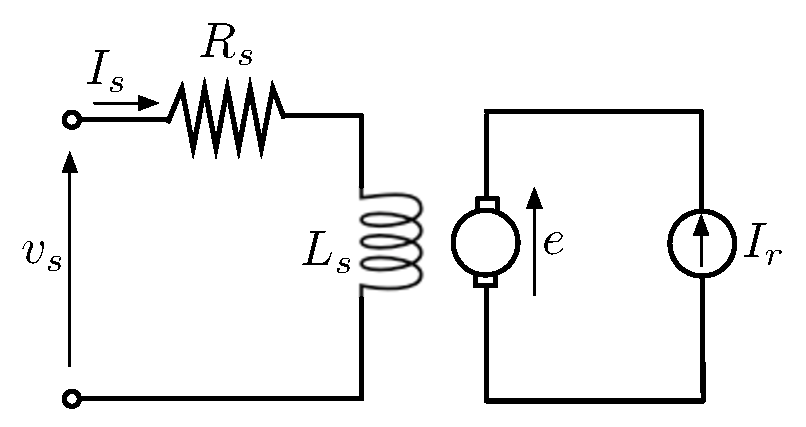
\includegraphics[height=4cm]{cominducteur}
\caption{ DC engine controlled by the stator}
\label{fig:cominducteur}
\end{center}
\end{figure}

\noindent The system has three state variables :
\begin{equation*} \begin{split}
x_1 &= \theta, \\
x_2 &= \dot{\theta}, \\
x_3 &= I_s. 
\end{split} \end{equation*}
The system inputs are the voltages at the terminals of the stator circuit $v_s$ and the external torque $T_a$ : 
\begin{equation*} \begin{split}
u_1 &= v_s, \\
u_2 &= T_a.
\end{split} \end{equation*}
The state-spaced model is written as follows :
\begin{equation*} \begin{split}
\dot x_1 &= x_2,\\
J\dot x_2 &= -h(x_2) + K_m I_r x_3 + u_2,\\
L_s\dot x_3 &= -R_s x_3 +u_1.
\end{split} \end{equation*}
\\
\noindent{\em DC engine controlled by the rotor.}

It's a DC engine whose stator current is provided by a constant current source ( figure \ref{fig:cominduit}):
\eqnn
I_s = constant
\eeqnn
\begin{figure}[htbp]
\begin{center}
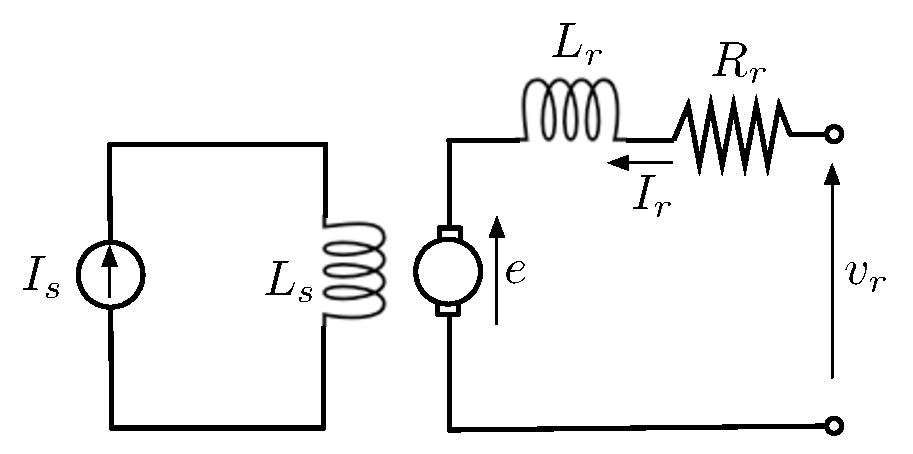
\includegraphics[height=4cm]{cominduit}
\caption{DC engine controlled by rotor}
\label{fig:cominduit}
\end{center}
\end{figure}
The system has three state variables :
\begin{equation*} \begin{split}
x_1 &= \theta, \\
x_2 &= \dot{\theta}, \\
x_3 &= I_r. 
\end{split} \end{equation*}
The system inputs are the voltage at the terminals of the rotor circuit $v_r$ and the external torque $T_a$ : 
\begin{equation*} \begin{split}
u_1 &= v_r, \\
u_2 &= T_a.
\end{split} \end{equation*}
The state-spaced model is written as follows :
\begin{equation*} \begin{split}
\dot x_1 &= x_2,\\
J\dot x_2 &= -h(x_2) + K_m I_s x_3 + u_2,\\
L_r\dot x_3 &= -R_r x_3 - K_e I_s x_2 + u_1.
\end{split} \end{equation*}
\\
\noindent{\em DC generator.}
The function of a generator is to convert mechanical power in electrical power \blue{delivered} by the rotor circuit on any load impedance of $Z_L$.

When this impedance is resistive ($R_L$),  the system has three state variables ( figure
\ref{fig:genDC})~: 
\begin{equation*} \begin{split} 
x_1 &= I_s, \\ x_2 &= I_r, \\ x_3 &= \omega.
\end{split} \end{equation*}
\begin{figure}[htbp]
\begin{center}
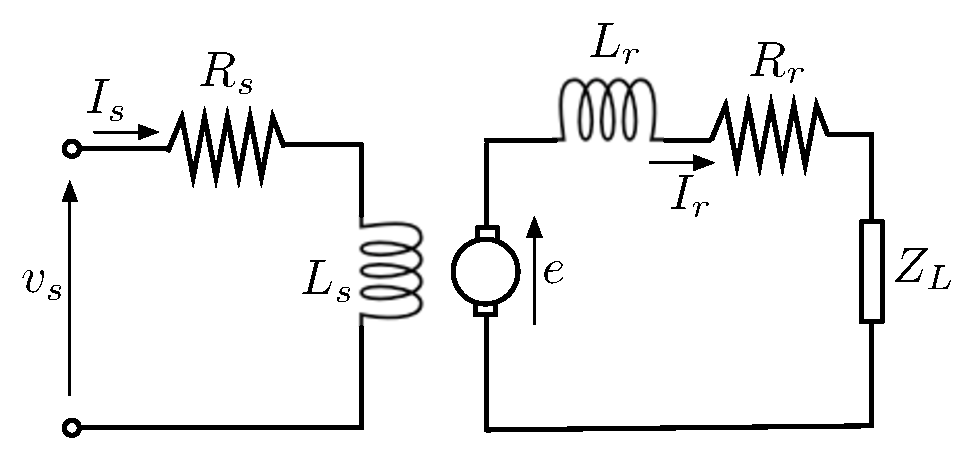
\includegraphics[height=4cm]{genDC}
\caption{ DC generator}
\label{fig:genDC}
\end{center}
\end{figure}
The system inputs are the voltage at the terminals of the stator circuit $v_s$ and the torque $T_a$ :
\begin{equation*} \begin{split}
u_1 &= v_s, \\
u_2 &= T_a.
\end{split} \end{equation*}
The state-spaced model is written as follows :
\begin{equation*} \begin{split}
L_s\dot x_1 &= -R_s x_1+ u_1, \\
L_r\dot x_2 &=  - (R_r +R_L) x_2 - K_e x_3 x_1,\\
J\dot x_3 &= -h(x_3) + K_m x_1x_2 + u_2.
\end{split} \end{equation*}


\section{Exercices}

\begin{exercice} {\bf \em Linear circuit}

Establish a state-spaced model of the linear circuit shown in figure  \ref{fig:circuitlin} with the applied voltage $e$ and the adjustable resistance $r$ as input variables. \qed
 \begin{figure}[htbp]
\begin{center}
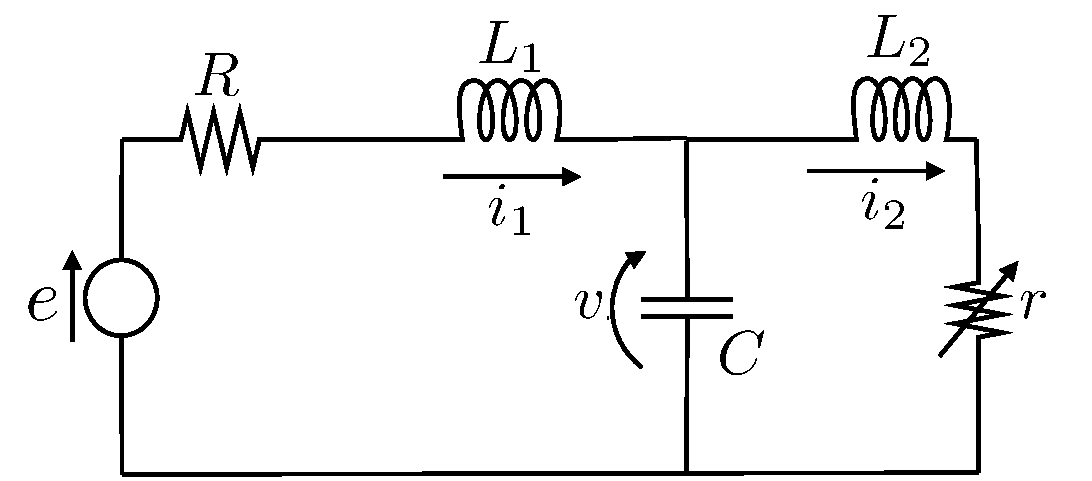
\includegraphics[height=4cm]{circuitlin}
\caption{Linear circuit}
\label{fig:circuitlin}
\end{center}
\end{figure}

\end{exercice}
\vv

\begin{exercice} {\bf \em Voltage doubler bridge}

The electrical diagram of a voltage doubler bridge is shown in figure \ref{fig:pont}. Establish the state-spaced model of the system assuming that all the dipoles are linear except the diodes. \qed
\begin{figure}[htbp]
\begin{center}
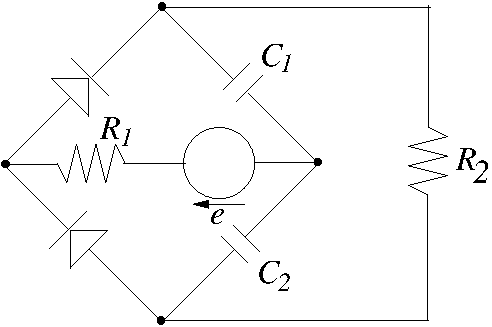
\includegraphics[height=4cm]{pont}
\caption{Voltage doubler bridge}
\label{fig:pont}
\end{center}
\end{figure}
\end{exercice}
\vv

\begin{exercice} {\bf \em Transformer}
The electrical diagram of a transformer is shown in figure
\ref{fig:transfo}.
\begin{figure}[htbp]
\begin{center}
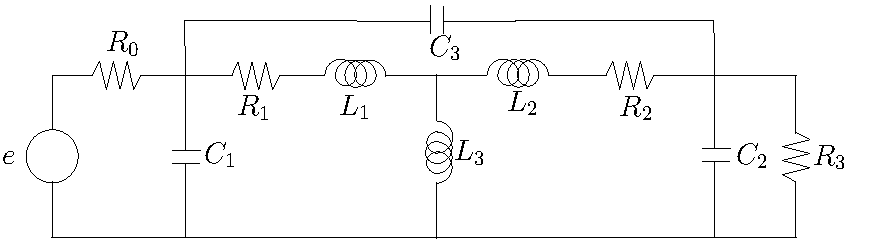
\includegraphics[height=3cm]{transfo}
\caption{Transformer equivalent circuit}
\label{fig:transfo}
\end{center}
\end{figure}
\begin{enumerate}
\item Has this electrical network some capacity \blue {mesh} and/or inductance \blue {cuts} ? 
 Explain your answer.
\item Establish the state-spaced model assuming that the dipoles are linear. \qed
\end{enumerate}
\end{exercice}
\vv

\begin{exercice}{\bf \em  A circuit with a tunnel diode}

A electrical circuit is described by the following state equations :
\eqnn
C \dot x_1 &=& -h(x_1)+x_2,\\
L\dot x_2 &=& -x_1-Rx_2 +u.
\eeqnn
$x_1$ is the voltage to the terminals of a linear capacity, $x_2$ is the current in a linear inductance, $h(x_1) = x^3_1 - 10 x^2_1 + 25 x_1$  
is the characteristic of a tunnel diode. Establish the circuit diagram. \qed
\end{exercice}
\vv

\begin{exercice}{\bf \em Electromechanical converter }

The device illustrated in figure \ref{fig:convem} transforms an electrical power provided
by the voltage source in a mechanical mouvement of translation.  It is made of a cylindrical steel core moving
longitudinally inside a solenoid. \qed
\begin{figure}[htbp]
\begin{center}
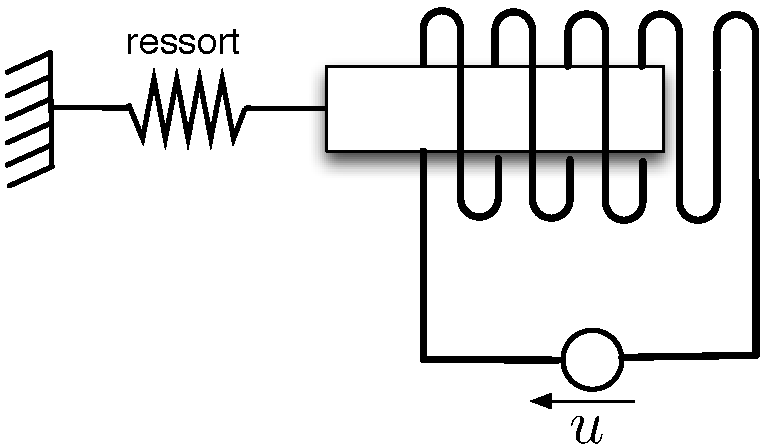
\includegraphics[height=3cm]{convem}
\caption{electromechanical converter}
\label{fig:convem}
\end{center}
\end{figure}

Suggest a state-spaced model of this system according to the following  modeling assumptions :
\begin{enumerate}
\item The core movement is forced to be linear by a slide.  The friction can be considered as viscous and linear.
\item The core is shorter than the solenoid.
\item The flow in the solenoid is a linear function of the length $h$ of the core part which is inside the solenoid.
\item The flow is a saturated monotonically increasing function of the current.
\item The spring is linear. \qed
\end{enumerate}
\end{exercice}

\begin{exercice}{\bf \em Clockwork motor}
A small motor used in watchmaking is presented in figure
\ref{fig:mothor}.  The stator is provided with field winding whose inductance
$L(\theta)$ is a sinusoidal function of the rotor angular position $\theta$.
\begin{figure}[htbp]
\begin{center}
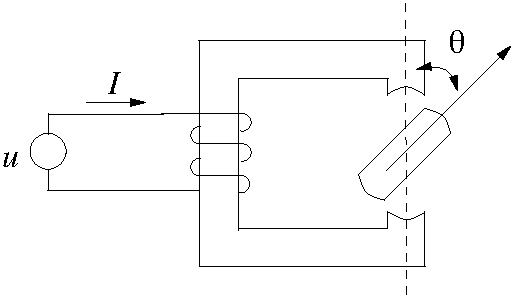
\includegraphics[height=40mm]{mothor}
\caption{Clockwork motor}
\label{fig:mothor}
\end{center}
\end{figure}
\begin{enumerate}
\item Suggest a model for the function $L(\theta)$ and compute the flow.
\item Establish the state-spaced model of the system assuming a linear viscous friction. The inputs are the 
voltage $u$ at the terminals of the inductor and the load torque $T_a$.
\item What has to be the waveform of the input signal $u$ when $T_a$ is constant and so that the rotor rotates at 
constant speed ?  \qed
\end{enumerate}
\end{exercice}
\newpage

%%%%%%%%%%%%%%%%%%%%%%%%%%%%%%%%%%%%%%%%%%%%%%%%%%
%%%%%%%%%%%%%%%%%%%%%%%%%%%%%%%%%%%%%%%%%%%%%%%%%%
%%%%%%%%%%%%%%%%%%%%%%%%%%%%%%%%%%%%%%%%%%%%%%%%%%
%%%%%%% PARTIE DE Nicolas Stevens    %%%%%%%%%%%%%%
%%%%%%%%%%%%%%%%%%%%%%%%%%%%%%%%%%%%%%%%%%%%%%%%%%
%%%%%%%%%%%%%%%%%%%%%%%%%%%%%%%%%%%%%%%%%%%%%%%%%%
%%%%%%%%%%%%%%%%%%%%%%%%%%%%%%%%%%%%%%%%%%%%%%%%%%

\begin{exercice}{\bf \em Unipolar of-phase synchronous machine} %Machine synchrone unipolaire diphasée.

This is a machine holding two stator windings (labelled $a$ and $b$) 
arrange in quadrature and a rotor winding (labelled $r$). 
The self and mutual inductances of the stator winding vary depending
on the angular position $\theta$ of the rotor according to the following laws : 
\eqnn 
L_a &=& L_o + L_1\cos 2\theta \nonumber \\ 
L_b &=& L_o - L_1\cos 2\theta \nonumber \\ 
L_{ab} &=& L_1 \sin 2\theta \nonumber 
\eeqnn 
The self inductance of the rotor $L_r$ is constant. The mutual 
inductances between the rotor and the stator windings are expressed in
terms of $\theta$ : 
\eqnn 
L_{ar} &=& L_2 \cos \theta \nonumber \\
L_{br} &=& L_2 \sin \theta \nonumber  
\eeqnn
\begin{enumerate} 
\item Establish the coupling equations of the electromechanics 
system (see Section 3.4) 
\item The rotor is supplied by a constant current source
$I_r$. Establish the state model of this machine when 
it works as an engine (you might need to use the example 3.3). \qed
\end{enumerate}
\end{exercice}
\vv

\begin{exercice}{\bf \em Elementary machine with two windings.}

Let's consider the elementary machine with two windings working as 
a generator, such as it is described in the example 3.3.
Denote how to revise the state equations under the following hypothesis : 
\begin{enumerate}
\item  The electric charge of the stator circuit is capacitive
\item  The rotor winding is closed using a short-circuit. \qed
\end{enumerate}
\end{exercice}
\vv

\begin{exercice}{\bf \em DC motor with self-excitation}

A DC motor with self-excitation is designed such as the stator 
current and the rotor current are supplied by the same power source
(see figure \ref{fig:autoex}). Establish the state model of the state model 
of this system using the tension source $u$ as the only input 
variable of this system. \qed
\begin{figure}[htbp]
\begin{center}
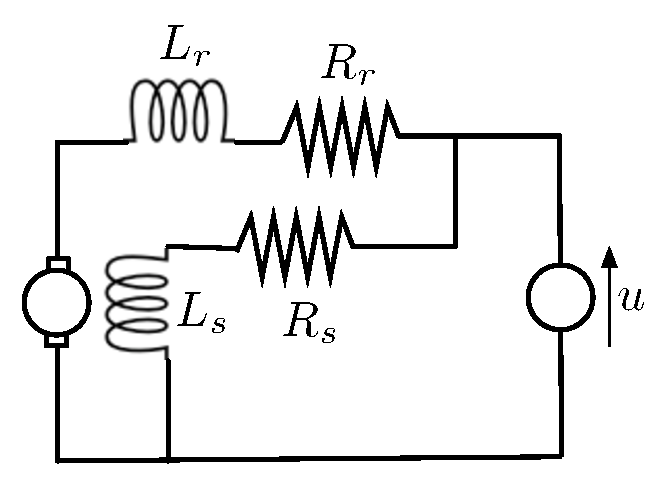
\includegraphics[height=4cm]{autoex}
\caption{DC motor with self-excitation}
\label{fig:autoex}
\end{center}
\end{figure}
\end{exercice}
\vv

\begin{exercice}{\bf \em DC generator with self-excitation}
Let's consider a DC generator with self-excitation. The rotor tension 
induced at constant rate is a {\em strictly  increasing and bounded} function 
depending on the excitation current $E(I_s)$ such as $E(0) >
0$. The generator provides a capacitive electric charge. 
The input control variable of the system is the rotation speed of 
the generator. 
\begin{enumerate}
\item Propose an analytical form for the function $E(I_s)$.
\item Propose a state model for this system.
\item Justify the existence of a non-zero residual voltage $E(0)$. \qed
\end{enumerate}
\end{exercice}
\vv

\begin{exercice}{\bf \em DC motor with off-center load}

A DC motor with independent excitations is controlled by the rotor current
driving an off-center load (the motor shaft do not pass through the 
center of mass of the load : indeed, there is an unbalanced effect)
through a transmission whose flexibility is significant. 
Propose a state model taking into account this features. 
\end{exercice}
\vv

\begin{exercice}{\bf \em DC-DC converters}

\begin{figure}[htbp]
\begin{center}
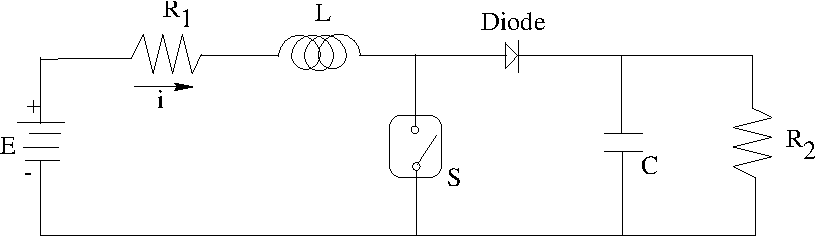
\includegraphics[width=85mm]{DCDC}
\caption{DC-DC converter}
\label{fig:DCDC}
\end{center}
\end{figure}
The circuit depicted at the figure above describes a DC-DC converter.  
The device labelled ``S" picture an electronic switch of type MOSFET 
which is open and close periodically.\\

Establish a state model of the system under the following modelling 
hypothesis :
\begin{itemize}
\item[a)] the voltage $E$ of the supply battery is constant
\item[b)] both resistances $R_1, R_2$, the inductance $L$ and the 
capacitor $C$ are linear
\item[c)] the input variable is the commutation frequency of the switch. \qed
\end{itemize} 
\end{exercice}



\end{document}
